\documentclass[11pt, a4paper]{article}
\usepackage[margin=0.5in]{geometry}
\usepackage{amsmath}
\usepackage{graphicx}
\graphicspath{ {./} }
\usepackage{mathtools}
\DeclarePairedDelimiter{\abs}{\lvert}{\rvert}
%\usepackage{parskip}
% equations coulde be %   default number of the equation on the rigth and equation centered 
%   leqno number on the left and equation centered %   fleqn number on the rigth and  equation on the left side
\newcommand{\solution}{ \noindent \textbf{Solution:}}
\newcommand{\problem}[1]{\textit{#1} \medskip}

% get rid of spacing after problem headers
\usepackage{titlesec}
%\titlespacing\subsection{0pt}{12pt plus 4pt minus 2pt}{0pt plus 2pt minus 2pt}
\titlespacing{\subsection}{0pt}{*3}{-\parskip}


\title{Combinatorial Optimization and Modern Heuristics: Assignment 1}
\author{Luke Floden\\
    \textsc{Computer Science \& Engineering}\\
	\and 
	Max Williams\\
    \textsc{Computer Science \& Engineering}\\
	}

\date{\today} 
\begin{document}
\maketitle

\section*{Chapter 1 Problems}

\subsection*{Problem 1(d)}

\problem{Find a cylinder with a given surface area A that has the largest volume $V$.}

\solution

Okay so this is just a basic b kinda maximization problem. Oh Also we could just make the cylinder
out of a bubble and physics would do gradient descent on the surface area... aph ph oh wait I got it
backwards. What am I doing? Microdosing might actually not be effectibe as tehy say.

So surface area is $2 \pi r^2 + 2 \pi r l$ where $r$ is the radius and $l$ is the length. Volume is
$ \pi r^2 l$. So given a fixed area, maximize the volume. Simply dimply.

\begin{align*}
    &2 \pi r^2 + 2 \pi r l = A\\
    &\text{maximize}\ \pi r^2 l\\
\end{align*}

Which is the same as maximizing $rl$. r and l are greater than 0. 

\begin{align*}
    &r^2 + r l = \frac{A}{2 \pi}\\
    &\text{maximize}\ r^2 l\\
\end{align*}

solve for $l$ and plug into maximization

\begin{align*}
    & l = \frac{A}{2 \pi r} - r\\
    &\text{maximize}\ \frac{Ar}{2 \pi} - r^3\\
\end{align*}

Taking the derivative of the cost function and finding where it is zero gives

\begin{align*}
    &\frac{A}{2 \pi} - 3r^2 = 0\\
    & 3r^2 = \frac{A}{2 \pi}\\
\end{align*}

TODO ask about what "instance" means at office hours

So uh at this point we should take a derivative or somethign. Dool.

Restrict r to be from 0 to inf, 

\subsection*{Problem 3}

\problem{Show that the neighborhood defined in Example 1.5 for the MST is exact.}

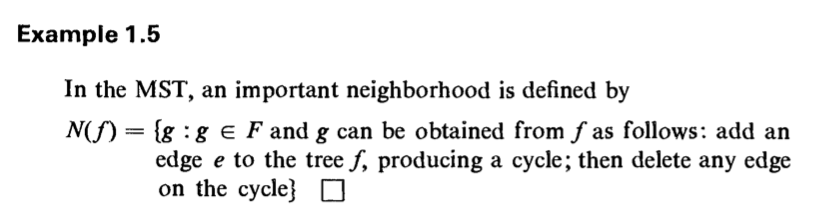
\includegraphics[scale=0.4]{ex15}

\solution

Oh god what. Exact? Fujk I sould have read the textbood.

\subsection*{Problem 6}

\problem{Suppose we are given a set $S$ containing $2n$ integers, and we wish to partition it into
two sets $S_1$ and $S_2$ so that $\abs{S_1}=\abs{S_2}=n$ and so that the sum of the numbers in $S_1$
is as close as possible to the sum of those in $S_2$. Let the neighborhood $N$ be determined by all
possible interchanges of two integers between $S_1$ and $S_2$. Is $N$ exact?}

\solution

Uhhhhh probably not, that algorithm sound insufficient to get a global solution, assuming that's the
same thing as exact.


\subsection*{Problem 9}

\problem{Let $f(x)$ be convex in $R^n$. Is $f(x+b)$, where $b$ is constant, convex in $R^n$?}

\solution

So we're gonna have to use the actual definition of convexity to make this more formal but I would
say yeah duh. Just translating the graph around is not going to change convexity. 

\subsection*{Problem 10}

\problem{Let $f(x_i)$ be a convex function of the single variable $x_i$. Then $g(x) = f(x_i)$ can also
be considered a function of $x \in R^n$. Is $g(x)$ convex in $R^n$?}

\solution

I don't really understand, isnt g just a copy of f? fok

\section*{Chapter 2 Problems}

\subsection*{Problem 8}

\problem{Show that the set of optimal point of an instance of LP is a convex set.}

\solution

Oooh I know that that's true! Well each boundary is a hyperplane, and the region bounded by
hyperplanes must be convex... that shouldn't be too hard to prove lol

\end{document}
